\chapter{Model Definition}\label{chp:model}

This chapter describes the design of our context graph structure with which we seek to develop a novel language model that is completely reconstructable, human-readable and updatable.\\
The model is based on a hierarchical structure of n-grams with a minimal representation of a sub-string containment order, augmenting n-grams with their contextual relationships and reducing their storage size. Frequency counts of n-grams can be calculated to perform various stochastic predictions within the contextual neighborhood of different parts of text.

%A major challenge of the structure is to handle the large number of possible n-grams and relationships between them, however we show that the amount of storage needed can be limited by representing longer n-grams using shorter ones. It is also a known fact that, following Zipf's Law, the frequency of most larger n-grams is not larger than 1 and by not storing these n-grams individually, we can already mitigate the space requirements by 60\% compared to a model storing every n-gram of the same length explicitly.

\section{Context Representation}
The key idea of the model is to represent all context relationships between frequent n-grams in a hierarchical deconstruction of the original corpus or input string. This approach is highly motivated by compression algorithms using a grammar or dictionary to represent their input while occupying less memory. These grammars do however not contain all context relationships between frequent n-grams and it is thus not possible to efficiently analyze them.\par

\noindent
The goal of this chapter is to find the minimal set of edges necessary to relate all frequent n-grams in a context graph and assign each node in the graph a frequency count, which can be used to calculate probabilities for transitions or nodes in the graph.

\noindent
We define the containment order on the set of all n-grams in the corpus of any length $n$. Represented as a graph, this relation will have all edges pointing from larger n-grams (super-strings) to the smaller n-grams (sub-strings) contained in them. Each n-gram or string is represented by a unique node connected to all of its sub-strings and their different parent contexts, giving a \emph{directed acyclic graph} (directed edges, no cycles).

%n-gram frequency counts can be used to calculate conditional probabilities of moving from one n-gram to another.

\dfn{Sub-String Relation}{
    The sub-string graph $G = (V, E)$ of a string $w \in \Sigma^*$ represent the \textbf{strict containment} order on sub-strings of $w$. Let $a < b$ denote the partial order on the set of sub-strings of $w$, ``$a$ is a strict sub-string of $b$'':
    %\begin{align*}
    %    a < b \iff \exists x,y \in \Sigma^*, (x, y) \neq (\epsilon, \epsilon): b = x \cdot a \cdot y
    %\end{align*}
    We may write $a \leq b$ to allow for $a = b$.
    The nodes of the graph are given by the set of all sub-strings of $w$ and the edges are given by the strict sub-string relation over these sub-strings:
    \begin{align*}
        V \coloneqq \{v \in \Sigma^+ \mid v \leq w \},\quad
        E \coloneqq \{(a, b) \in V^2 \mid a < b \}
    \end{align*}
    Note that $V$ includes the original string $w$.
    
    We will denote the string representation of a node $v \in V$ as $\texttt{string}(v)$ and refer to them as n-grams of degree $n = |\texttt{string}(v)|$
}

\noindent
As a result, the graph of the sub-string relation contains all the edges directly connecting super-strings with all of their sub-strings.

\noindent
For large corpora, this structure would grow far too large to be practical as the worst-case space complexity for storing the nodes is quadratic. The number of possible sub-strings of length $n$ within a string of length $N$ is $N - n + 1$. For all lengths $n$ up to $N$, this amounts to $\sum_{n=1}^{N}{N-n+1} = \frac{N(N + 1)}{2}$ many sub-strings to a string of length $N$ for which nodes need to be stored.

\noindent
For each node of length $n$ the sub-string relation stores an edge to each of its substrings, of which there are $\frac{n(n + 1)}{2}$ by the same argument as above.

\noindent
The total number of edges will be the sum of all edges for every node of length $n$.
\begin{align*}
|E| &= \sum_{n=1}^{N}{(N - n + 1)\frac{n^2 + n}{2}} = \frac{1}{2}\sum_{n=1}^{N}{Nn^2 - n^3 + (N + 1)n}
\end{align*}
with $s(k) \coloneqq \sum_{n=1}^{N}{n^k}$ and $s(3) = {s(1)}^2$ (Faulhaber's formula~\cite{orosi2018simple}) we can follow
\begin{align*}
2|E| &= N^2s(2) - s(3) + N(N + 1)s(1) =
N^2s(2) - \frac{{\left(N(N+1)\right)}^2}{4} + \frac{\left(N(N+1)\right)^2}{2}\\
&= N^2s(2) + s(3) = \frac{N^3(N+1)(2N+1)}{6} + \frac{N^2{(N+1)}^2}{4}
\end{align*}
resulting in a worst case space complexity of $O(N^5)$ for the number of edges in the complete sub-string graph. We are going to show how to reduce the number of edges we need to store, while maintaining all the paths between substrings and keep sub-strings connected with their contexts.

\section{Reducing the Number of Edges}\label{sec:edge_reduction}

We are only concerned about representing context relationships with this structure. We can perform a \textbf{transitive reduction} on the sub-string relation graph by only preserving the minimal set of edges needed to keep all paths between any two n-grams.

\dfn{Transitive Reduction}{
    The transitive reduction $G_T = (V, E_T)$ of a graph $G$ with no cycles is the result of removing all edges from $G$ for which there exists a longer path connecting their endpoints. The graph $G_T$ has the properties
    \begin{enumerate}[label= (\roman*)]
        \item\label{itm:first} There is a path between nodes $u$ and $v$ in $G_T$ if and only if there is a path between $u$ and $v$ in $G$. The graphs have the same \textit{reachability} relation.
        \item There is no graph with fewer edges than $G_T$ fulfilling property~\ref{itm:first}
    \end{enumerate}
}
In the transitive reduction of the sub-string relation of a corpus, edges can be omitted if there exists another path between the endpoints. This way we can still find all sub-strings of any given node and can also reach all possible contexts of a string. The reachability of the transitively reduced relation is the same.

This allows us to store only a subset of the edges as we can reuse the connections from other related strings. The only downward edges that need to be stored for each node are to those sub-strings which can not be contained in any larger sub-string. Under the assumption that nodes for \emph{all} possible sub-strings exist, there are only $2$ sub-strings of each string with this property, the prefix and the postfix of length $n-1$.
\begin{table}[!ht]
    \ttfamily
    \centering
    $\expanded{\noexpand\begin{tblr}{
        \newcell{1}{1}{5},
        \newcell{2}{2}{5},
        hspan = even,
    }}
    prefix&&&&&\quad\\
    \quad&postfix&&&&
    \end{tblr}$
\end{table}

In the transitive reduction, still every sub-string is reachable from every node, by travelling over the paths iteratively. However, as we only have to store a constant number edges for each node, the number of edges in the sub-string relation is reduced to $N(N + 1)$ or $O(N^2)$.

\section{Reducing the Number of Nodes}\label{sec:frequency_reduction}
The goal of the model is to connect frequent sub-strings of the corpus with their various contexts and to derive probabilities for different contexts of a given string. For this we do not need to store dedicated nodes for n-grams which occur only in a single context, as it can be represented in the context node and storing an additional node would be redundant. Root super-strings represent training examples and will have no parents. A constraint to formalize this could be:\par
\emph{Nodes should not have exactly one parent}.

This can however not always be fulfilled, as some frequent child nodes of a string may overlap, while other children do not have overlaps. There are multiple ways to deal with this, and we have chosen to create new nodes for the overlapping portions to avoid repeating surrounding, non-overlapping contexts. Now the constraint becomes:\par
\emph{Nodes must not have exactly one parent while having no overlapping children.}

\noindent To define this more formally, we are going to make another extension to the structure with \emph{string partitions}. Instead of only linking each node with the minimal set of smaller nodes required by the transitive reduction, we require each node to contain the minimal set of partitions of its string, represented using all child nodes from the transitively reduced containment graph.

\newpage
\begin{figure}
    \centering
    %\hspace{-1cm}
    \begin{subfigure}[c]{0.48\textwidth}
        %\centering
        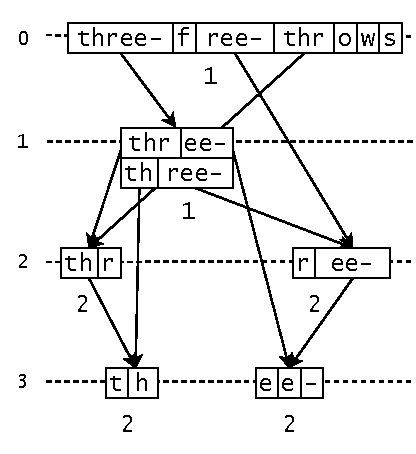
\includegraphics[scale=0.68, width=\textwidth]{images/three_free_throws.pdf}
    \end{subfigure}
    \hfill
    \begin{subfigure}[c]{0.50\textwidth}
        %\centering
        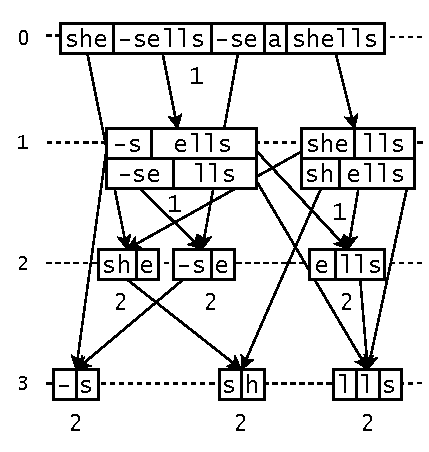
\includegraphics[scale=0.68, width=\textwidth]{images/she-sells-seashells.pdf}
    \end{subfigure}
    \caption{Substring partition graphs of the strings \texttt{three-free-throws} and \texttt{she-sells-seashells}. Nodes show partitions and frequency counts. Unigram nodes are omitted and levels are annotated by depth.}
\end{figure}

\dfn{Partition Graph}{
    Each node $n$ contains a minimal set of partitions $\texttt{parts}(n)$, where each partition $p_i$ is a list of $n_i$ child nodes, together representing the entire string of $n$: $\texttt{string}(n)$:
    \begin{align*}
        p_i \coloneqq \left(v_{i1}, \ldots, v_{in_i}\right) && \textit{such that} && \prod_{1 \leq j \leq n_i} \texttt{string}(v_{ij}) = \texttt{string}(n)
    \end{align*}
    (where $\cdot$ denotes string concatenation)\\
    in such a way that every direct child in the transitively reduced sub-string graph $G_T$ is present in one of the partitions:
    \begin{align*}
        \forall c \in children_{G_T}(n): \exists p \in \texttt{parts}(n): c \in p
    \end{align*}
    This means every node in the graph of partitions $G_P$can reach all of its sub- and super-strings, since the child partitions contain all the edges necessary for the transitive reduction of the complete sub-string relation.
}\label{def:partitions}

\noindent Since one partition can not contain two overlapping children, we can follow that any node with overlapping children in $G_T$ also has more than one partition. The nodes contained in the child partitions of each node contain all nodes necessary to reach every existing sub-string node and additionally some padding at the outer ends, so that each partition represents the whole string.\\
While this is not necessarily required, as the padding nodes are also reachable from one of the other nodes, it makes the formalism a bit simpler, as each partition represents the same string.

\noindent
In this formulation the criterion for each node can be written as:
\[
    \texttt{parents}(node) \neq 1 \lor \texttt{parts}(node) \neq 1
\]

When applying this, many nodes of the original substring relation are removed and our assumption from~\ref{sec:edge_reduction} that all sub-string nodes exist does no longer hold. In the partition graph, we can see that no border between two adjacent sub-string nodes can occur in two different partitions. Any sequence of nodes in any two partitions with a border at the same token location will always be expressed as a single larger node containing the sequences as its child partitions instead, following the constraints from the transitive reduction~\ref{sec:edge_reduction}. By removing those nodes that do not follow the above constraints, it becomes impossible for any two partitions to have a node border at the same token position.

From this follows that any node length $n$ can have at most $n-1$ borders between child nodes in all of its partitions and thus a number of child nodes in the order of $O(n)$. This gives us an upper bound for the number of edges in the partition graph:
\begin{align*}
\sum_{n=1}^{N}{(N - n + 1)n} &= \sum_{n=1}^{N}{Nn - n^2 + n} = N^2s(1) - s(2) + s(1) = O(N^4)
\end{align*}

This upper bound however ignores the fact that a higher number of nodes generally allows for more compression and ultimately results in less edges per node, illustrated by the extreme case where each node can have at most 2 significant children in the transitive reduction graph~\ref{sec:edge_reduction}. Such an edge space complexity can only be reached if there is a minimal amount of repetition in the input, which would also reduce the number of total nodes.

\section{Maximum number of nodes over an alphabet}

The total number of possible strings length $n$ which can be built over an alphabet of $k$ symbols is $k^n$. This means that for small $n$, the number of possible individual nodes may much smaller than is indicated by the number of possible sub-strings: $N - n + 1$, as they are limited by the number of unigrams or atomic tokens $k$. With respect to this, the equation for the total number of possible nodes in a string length $N$ over $k$ symbols becomes:
\begin{align*}
    |V| = \sum_{n=1}^N{\min\{k^n, N - n + 1\}}
\end{align*}

\noindent
Both the functions are monotonic with respect to $n$, $k^n$ being an increasing function and $N - n + 1$ is a decreasing function.
\newpage
\noindent
To sum only the minimum value of both functions, we can split the sum into two parts at their intersection point $n^*$, where
\begin{equation} \label{eq:1}
    k^{n^*} = N - n^* + 1 \Leftrightarrow \log_k(k^{n^*} - n^*) = \log_k(N + 1)
\end{equation}

With the intersection point, can then express the sum as two parts, summing each side of the intersection independently:
\begin{align} \label{eq:2}
    |V| = \sum_{n \in \interval{1}{n^*}}{k^n} + \sum_{n \in \interval[open left]{n^*}{N}}{N - n + 1}
\end{align}
%!\ref{eq:1}% 

Because equation~\ref{eq:1} is a transcendental function, there is no algebraic solution for $n^*$, but we can get a sufficient estimate by utilising that
\begin{align*}
    \log(s + t) = \log(s) + \log(1 + \frac{t}{s}) \approx \log(\max\{s, t\}), \text{ if } |s - t| \gg 0
\end{align*}
\noindent
which allows us to rewrite equation~\ref{eq:1} as 
\begin{align*}
    \log_k(k^{n^*} - n^*) = \log_k(N + 1) &\approx \log_k(\max\{k^{n^*}, - n^*\}) = n^*, \text{ if } k^{n^*} \gg -n^*
\end{align*}
giving an approximation of $n^* \approx \log_k(N + 1)$ for large $N$, sufficient for our purposes. We have verified this intersection point numerically using Newton's method for approximating roots of non-linear equations.

\noindent
Then, we approximate equation~\ref{eq:2} with its integral form
\begin{align*}
    |V| &\approx \int_{1}^{n^*}{k^n}\diff n + \int_{n^*}^{N}{\left(N - n + 1\right)}\diff n\\
        &= {\left[\frac{k^n}{\ln(k)} \right]}_{1}^{n^*} + {\left[(N + 1)n - \frac{n^2}{2} \right]}_{n^*}^{N}
        = \frac{k^{n^*} - k}{\ln(k)} + \frac{N^2}{2} + N - (N + 1)n^* + \frac{{n^*}^2}{2}
\end{align*}
and replacing $n^* = \log_k(N + 1)$
\begin{align*}
    |V| \approx \frac{N + 1 - k}{\ln(k)} + \frac{N^2}{2} + N - (N + 1)\log_k(N + 1) + \frac{{\log_k(N+1)}^2}{2}
\end{align*}

giving an asymptotic order of $O(N^2 + \log_k(N)^2)$ for the total number of possible sub-strings for a corpus of length $N$ over an alphabet of $k$ tokens. Giving an even lower upper bound for the worst case for the number of nodes required to represent a specific string of length $N$ over $k$ different tokens.

\newpage
\begin{figure}
\centering
\hspace{-1cm}
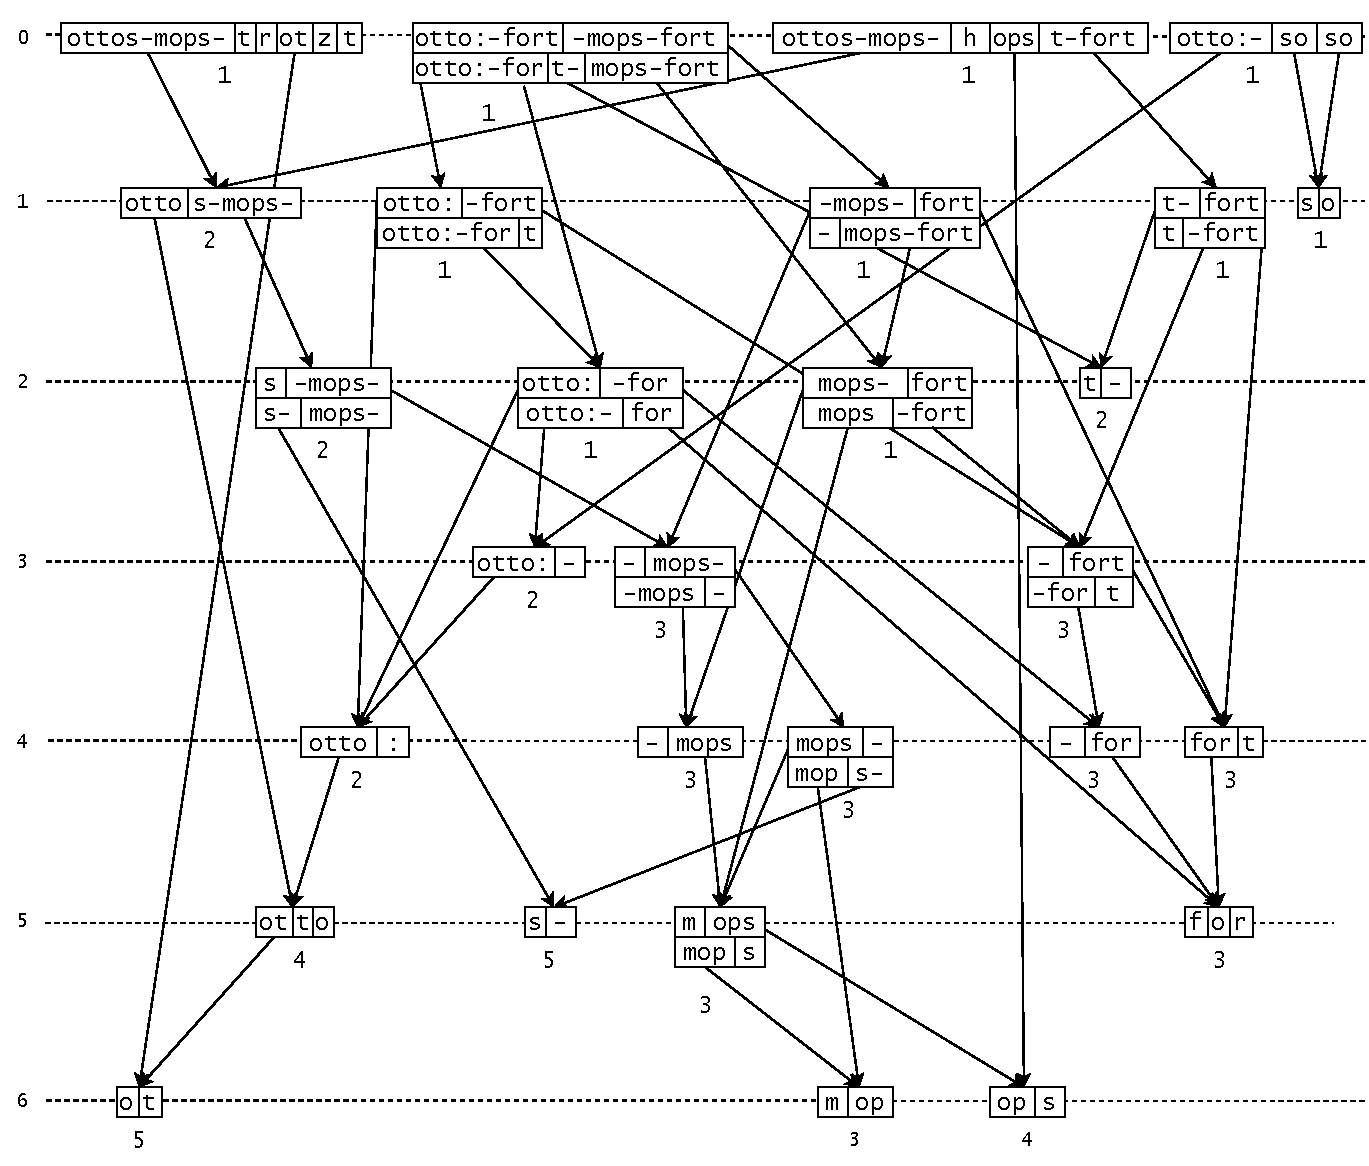
\includegraphics[scale=0.68]{images/substring_graph_counted.pdf}
\caption{A complete transitively reduced sub-string partition graph of four example sentences. Nodes show partitions and frequency counts. Unigram nodes are omitted and levels are annotated by depth.}
\end{figure}


\section{Reconstructing Training Data}

Of course, it is generally possible that the same sub-string appears at different positions in a larger string, for example $prefix = postfix$. To account for this in the representation, we associate each edge in the relation with the relative position of the child in the super-string. The resulting graph has edge labels in the form of sets of these positions.

\dfn{Offset Relation}{
    The offset relation $\texttt{offsets}(e): E_T \rightarrow \mathcal{P}(\NN)$ assigns each edge of the reduced sub-string relation $G_T$ the set of offsets where the sub-string occurs in the super-string.
    \begin{align*}
        \texttt{offsets}(x, y) \coloneqq \{|a| \mid \forall a, b \in \Sigma^*: \texttt{string}(x) = a \cdot \texttt{string}(y) \cdot b\}
    \end{align*}
    where $\text{string}(\cdot)$ gives the string associated with a node in $G_T$. Each offset is defined as the number of tokens preceding the sub-string in the super-string.
}
With the offset relation in place we are able to reconstruct the original string from the reduced sub-string relation $G_T$, as we now know where each sub-string needs to be placed. Because nodes in $G_T$ must be connected to all of their sub-strings, we are able to reach each of the tokens represented by the node. With the offset relation, providing us with a relative position of each sub-string, we can also derive the absolute position of each token and reconstruct the input.

For any node $v$ we can reconstruct its corresponding string $\texttt{string}(v)$ if we know the strings of its children. If a node has no children it shall represent a single token, drawn from a dictionary. These nodes represent unigrams, where $|\texttt{string}(v)| = 1$. Any larger nodes must have these nodes as sub-strings and thus a path to these unigram nodes. Each path is annotated with offsets on each edge, and thus we can reconstruct the token for each position of a node's string.

\section{Counting n-gram Frequencies}

For statistical predictions about surrounding contexts frequency counts can be used to calculate the probability of each frequent context:
\dfn{Frequency Counts}{
    $\texttt{count}(v): V \rightarrow \NN$ assigns each string in the sub-string relation $G_T$ the number of its occurrences in the corpus.
    
    The frequency counts can be used in an N-Gram model to make predictions about surrounding tokens of a given string:
    \[
        P(c \mid n) = \frac{\texttt{count}(c)}{\texttt{count}(n)}
    \]
}
The counts represent the number of occurrences of each sub-string in the training corpus $T$. Each of these occurrences in $T$ can be represented by a position index able to reference any position in the given corpus. For example, a corpus consisting of a single string, could reference each sub-string's occurrence by its offset $p$ from the start of the string. A corpus composed of multiple separate strings could use a two-dimensional index $(s, p)$ of string index and position to reference the occurrence of some sub-string.

In a given graph these occurrences can easily be counted by passing all occurrences from top to bottom. It requires a bit of care since multiple different contexts can point to the same child at the same position (for example \texttt{lls} is a child of \texttt{-sells} and \texttt{ells} but in both instances occurs at the same position), however this is easily handled by tracing the global position for each node and only counting unique instances.

\paragraph{Counting Algorithm}
A simple algorithm to calculate the counts for each node can be given by a recursive breadth-first traversal of the graph, counting every unique occurrence for each node and passing them on to the child nodes.

For each node $n$ we collect a set of occurrence positions $O_n$, where the root nodes are assigned a single position: $O_s \coloneqq \{(s, 0)\}$. Every child node will now construct its set of occurrences from each of it parents occurrences and its offset in the parent:
\[
    O_n \coloneqq \{ (s, i + r) \mid (s, i) \in O_p, p \in \texttt{parents}(n), r \in
    \texttt{offsets}(p, n)\}
\]
In words, the occurrences of a node $n$ are given by its relative positions in the occurrences of all of its parents. The count of each node is then given by the number of occurrences: $\texttt{count}(n) \coloneqq |O_n|$.


\begin{center}
    ---
\end{center}
\noindent
Now that we understand the structure of the model, we can define the algorithm for constructing it from a raw text corpus.

%\dfn{Children \& Parents}{
%    The set of directly adjacient sub-string-smaller nodes are called \textit{children} of $v \in V$:
%    \begin{align*}
%        \text{Children}(v) \coloneqq \{ x \in N(v) \mid x < v \}
%    \end{align*}
%    where $N(v)$ is the neighborhood of $v$.
%    Complementary to this we define the parents of a node as its directly adjacient larger nodes.
%    \begin{align*}
%        \text{Parents}(v) \coloneqq \{ x \in N(v) \mid v < x \}
%    \end{align*}
%    As the sub-string relation is transitive, the sets are disjoint $\text{Parents}(v) \cap \text{Children}(v) = \emptyset$ and there are no cycles in the relation graph.
%}
%
%\dfn{Context Function}{
%    The contexts $\text{Ctx}(v)$ of a given node $v \in V$ are given by the set of nodes larger than $v$ in the sub-string relation:
%    \begin{align*}
%        \text{Ctx}(v) \coloneqq \{x \in V \mid v < x \}
%    \end{align*}
%    Complementary to this we define the set of sub-strings $\text{Sub}(v)$ of a node as the set of smaller nodes:
%    \begin{align*}
%        \text{Sub}(v) \coloneqq \{x \in V \mid x < v \}
%    \end{align*}
%    Each of these sets forms a subgraph of the sub-string relation, by adding the edges from the (reduced) sub-string relation:
%    \begin{align*}
%        E_{\text{Ctx}}(v) &\coloneqq \{(x, y) \in E_T \mid x \in \text{Ctx}(v) \land y \in \text{Ctx}(v)\}\\
%        E_{\text{Sub}}(v) &\coloneqq \{(x, y) \in E_T \mid x \in \text{Sub}(v) \land y \in \text{Sub}(v)\}\\
%        G_{\text{Ctx}}(v) &\coloneqq (\text{Ctx}(v), E_{\text{Ctx}}(v))\\
%        G_{\text{Ctx}}(v) &\coloneqq (\text{Sub}(v), E_{\text{Sub}}(v))\\
%    \end{align*}
%}